\chapter{Virtauslaskenta}

Virtauslaskenta on verkkoteorian osa-alue,
jonka keskeinen ongelma on verkon maksimivirtauksen laskeminen.
Tässä luvussa tutustumme ensin algoritmiin,
jonka avulla voi laskea verkon maksimivirtauksen,
ja sen jälkeen perehdymme erilaisiin virtauslaskennan sovelluksiin.

\section{Käsitteitä}

Oletamme, että annettuna on suunnattu,
painotettu verkko, 
jossa on valittu tietty alkusolmu ja loppusolmu.
Käytämme esimerkkinä seuraavaa verkkoa,
jossa solmu 1 on alkusolmu ja solmu 6 on loppusolmu:

\begin{center}
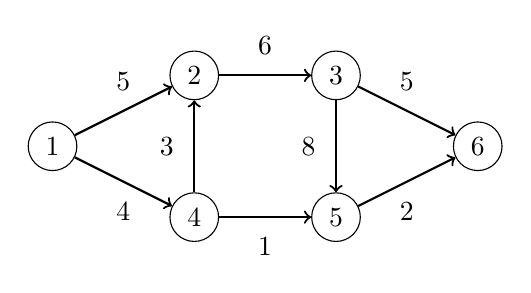
\begin{tikzpicture}[scale=0.9]
\node[draw, circle] (1) at (1,2) {$1$};
\node[draw, circle] (2) at (3,3) {$2$};
\node[draw, circle] (3) at (5,3) {$3$};
\node[draw, circle] (4) at (7,2) {$6$};
\node[draw, circle] (5) at (3,1) {$4$};
\node[draw, circle] (6) at (5,1) {$5$};
\path[draw,thick,->] (1) -- node[font=\small,label=5] {} (2);
\path[draw,thick,->] (2) -- node[font=\small,label=6] {} (3);
\path[draw,thick,->] (3) -- node[font=\small,label=5] {} (4);
\path[draw,thick,->] (1) -- node[font=\small,label=below:4] {} (5);
\path[draw,thick,->] (5) -- node[font=\small,label=below:1] {} (6);
\path[draw,thick,->] (6) -- node[font=\small,label=below:2] {} (4);
\path[draw,thick,<-] (2) -- node[font=\small,label=left:3] {} (5);
\path[draw,thick,->] (3) -- node[font=\small,label=left:8] {} (6);
\end{tikzpicture}
\end{center}

\subsubsection{Maksimivirtaus}

Virtaus (\textit{flow})
lähtee liikkeelle alkusolmusta ja päätyy loppusolmuun.
Kunkin kaaren paino on kapasiteetti,
joka ilmaisee, kuinka paljon virtausta kaaren
kautta voi kulkea.
Kaikissa solmuissa alku- ja loppusolmua lukuun ottamatta
tulevan ja lähtevän virtauksen on oltava yhtä suuri.

Maksimivirtaus (\textit{maximum flow}) on suurin
mahdollinen virtaus verkossa.
Esimerkkiverkossa maksimivirtauksen suuruus on 7:

\begin{center}
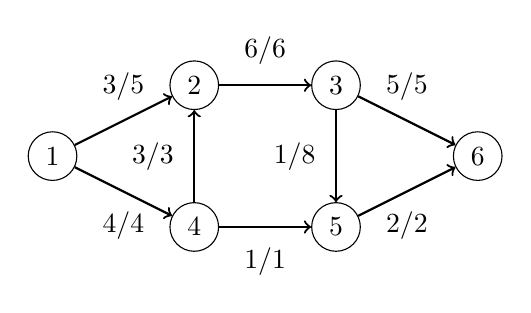
\begin{tikzpicture}[scale=0.9]
\node[draw, circle] (1) at (1,2) {$1$};
\node[draw, circle] (2) at (3,3) {$2$};
\node[draw, circle] (3) at (5,3) {$3$};
\node[draw, circle] (4) at (7,2) {$6$};
\node[draw, circle] (5) at (3,1) {$4$};
\node[draw, circle] (6) at (5,1) {$5$};
\path[draw,thick,->] (1) -- node[font=\small,label=3/5] {} (2);
\path[draw,thick,->] (2) -- node[font=\small,label=6/6] {} (3);
\path[draw,thick,->] (3) -- node[font=\small,label=5/5] {} (4);
\path[draw,thick,->] (1) -- node[font=\small,label=below:4/4] {} (5);
\path[draw,thick,->] (5) -- node[font=\small,label=below:1/1] {} (6);
\path[draw,thick,->] (6) -- node[font=\small,label=below:2/2] {} (4);
\path[draw,thick,<-] (2) -- node[font=\small,label=left:3/3] {} (5);
\path[draw,thick,->] (3) -- node[font=\small,label=left:1/8] {} (6);
\end{tikzpicture}
\end{center}

Merkintä $v/k$ kaaressa tarkoittaa,
että kaaressa kulkee virtausta $v$
ja kaaren kapasiteetti on $k$.
Virtauksen suuruus on 7, koska alkusolmusta
lähtevä virtaus on $3+4=7$ ja loppusolmuun
saapuva virtaus on $5+2=7$.

Huomaa, että jokaisessa välisolmussa tulevan ja
lähtevän virtauksen määrä on sama.
Esimerkiksi solmuun 2 tulee virtausta $3+3=6$ yksikköä solmuista 1 ja 4
ja siitä lähtee virtausta $6$ yksikköä solmuun 3.

Virtaus 7 on verkon maksimivirtaus, koska verkon
rakenteesta johtuen ei ole tapaa
kuljettaa enempää virtausta verkossa.

\subsubsection{Minimileikkaus}

Leikkaus (\textit{cut}) jakaa verkon solmut
kahteen osaan niin, että alkusolmu ja loppusolmu
ovat eri osissa.
Leikkauksen paino on niiden kaarten yhteispaino,
jotka kulkevat alkusolmun osasta loppusolmun osaan.

Minimileikkaus (\textit{minimum cut})
on leikkaus, jonka paino on pienin mahdollinen.
Esimerkkiverkossa minimileikkaus on painoltaan 7:

\begin{center}
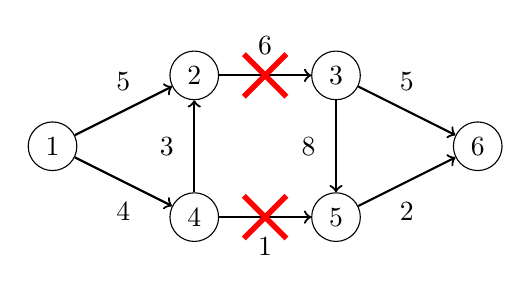
\begin{tikzpicture}[scale=0.9]
\node[draw, circle] (1) at (1,2) {$1$};
\node[draw, circle] (2) at (3,3) {$2$};
\node[draw, circle] (3) at (5,3) {$3$};
\node[draw, circle] (4) at (7,2) {$6$};
\node[draw, circle] (5) at (3,1) {$4$};
\node[draw, circle] (6) at (5,1) {$5$};
\path[draw,thick,->] (1) -- node[font=\small,label=5] {} (2);
\path[draw,thick,->] (2) -- node[font=\small,label=6] {} (3);
\path[draw,thick,->] (3) -- node[font=\small,label=5] {} (4);
\path[draw,thick,->] (1) -- node[font=\small,label=below:4] {} (5);
\path[draw,thick,->] (5) -- node[font=\small,label=below:1] {} (6);
\path[draw,thick,->] (6) -- node[font=\small,label=below:2] {} (4);
\path[draw,thick,<-] (2) -- node[font=\small,label=left:3] {} (5);
\path[draw,thick,->] (3) -- node[font=\small,label=left:8] {} (6);

\path[draw=red,thick,-,line width=2pt] (4-.3,3-.3) -- (4+.3,3+.3);
\path[draw=red,thick,-,line width=2pt] (4-.3,3+.3) -- (4+.3,3-.3);
\path[draw=red,thick,-,line width=2pt] (4-.3,1-.3) -- (4+.3,1+.3);
\path[draw=red,thick,-,line width=2pt] (4-.3,1+.3) -- (4+.3,1-.3);
\end{tikzpicture}
\end{center}

Tässä leikkauksessa alkusolmun osassa ovat solmut $\{1,2,4\}$
ja loppusolmun osassa ovat solmut $\{3,5,6\}$.
Alkusolmun osasta loppusolmun osaan kulkevat
kaaret $2 \rightarrow 3$ ja $4 \rightarrow 5$,
joiden yhteispaino on $6+1=7$.

~\\
\noindent
Ei ole sattumaa, että yllä olevassa verkossa
sekä maksimivirtauksen suuruus
että minimileikkauksen paino on 7.
Virtauslaskennan keskeinen tulos on,
että verkon maksimivirtaus ja
minimileikkaus
ovat \textit{aina} yhtä suuret,
eli käsitteet kuvaavat saman asian
kahta eri puolta.

Seuraavaksi tutustumme Ford-Fulkersonin
algoritmiin, jolla voi etsiä verkon
maksimivirtauksen ja
minimileikkauksen.
Algoritmi auttaa myös ymmärtämään,
\textit{miksi} maksimivirtaus ja
minimileikkaus ovat yhtä suuret.

\section{Ford-Fulkersonin algoritmi}

Ford-Fulkersonin algoritmi etsii verkon maksimivirtauksen.
Algoritmin ideana on aloittaa tilanteesta,
jossa virtaus on 0, ja etsiä sitten verkosta polkuja,
jotka tuottavat siihen lisää virtausta.
Kun mitään polkua ei enää pysty muodostamaan,
maksimivirtaus on valmis.

Algoritmi käsittelee verkkoa muodossa,
jossa jokaiselle kaarelle on vastakkaiseen
suuntaan kulkeva pari.
Kaaren paino kuvastaa, miten paljon
lisää virtausta sen kautta pystyy vielä kulkemaan.
Aluksi alkuperäisen verkon kaarilla on
painona niiden kapasiteetti
ja käänteisillä kaarilla on painona 0.

\begin{samepage}
Esimerkkiverkosta syntyy seuraava verkko:

\begin{center}
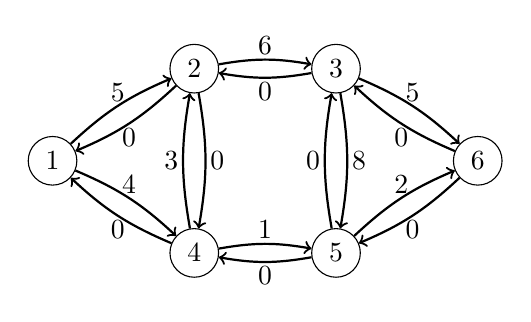
\begin{tikzpicture}[scale=0.9,label distance=-2mm]
\node[draw, circle] (1) at (1,1.3) {$1$};
\node[draw, circle] (2) at (3,2.6) {$2$};
\node[draw, circle] (3) at (5,2.6) {$3$};
\node[draw, circle] (4) at (7,1.3) {$6$};
\node[draw, circle] (5) at (3,0) {$4$};
\node[draw, circle] (6) at (5,0) {$5$};

\path[draw,thick,->] (1) edge [bend left=10] node[font=\small,label=5] {} (2);
\path[draw,thick,->] (2) edge [bend left=10] node[font=\small,label=below:0] {} (1);
\path[draw,thick,->] (2) edge [bend left=10] node[font=\small,label=6] {} (3);
\path[draw,thick,->] (3) edge [bend left=10] node[font=\small,label=below:0] {} (2);
\path[draw,thick,->] (3) edge [bend left=10] node[font=\small,label=5] {} (4);
\path[draw,thick,->] (4) edge [bend left=10] node[font=\small,label=below:0] {} (3);
\path[draw,thick,->] (1) edge [bend left=10] node[font=\small,label=4] {} (5);
\path[draw,thick,->] (5) edge [bend left=10] node[font=\small,label=below:0] {} (1);
\path[draw,thick,->] (5) edge [bend left=10] node[font=\small,label=1] {} (6);
\path[draw,thick,->] (6) edge [bend left=10] node[font=\small,label=below:0] {} (5);
\path[draw,thick,->] (6) edge [bend left=10] node[font=\small,label=2] {} (4);
\path[draw,thick,->] (4) edge [bend left=10] node[font=\small,label=below:0] {} (6);
\path[draw,thick,->] (5) edge [bend left=10] node[font=\small,label=left:3] {} (2);
\path[draw,thick,->] (2) edge [bend left=10] node[font=\small,label=right:0] {} (5);
\path[draw,thick,->] (3) edge [bend left=10] node[font=\small,label=right:8] {} (6);
\path[draw,thick,->] (6) edge [bend left=10] node[font=\small,label=left:0] {} (3);
\end{tikzpicture}
\end{center}
\end{samepage}

\subsubsection{Algoritmin toiminta}

Ford-Fulkersonin algoritmi etsii verkosta joka vaiheessa polun,
joka alkaa alkusolmusta,
päättyy loppusolmuun ja jossa jokaisen kaaren
paino on positiivinen.
Jos vaihtoehtoja on useita, mikä tahansa valinta kelpaa.

Esimerkkiverkossa voimme valita vaikkapa seuraavan polun:

\begin{center}
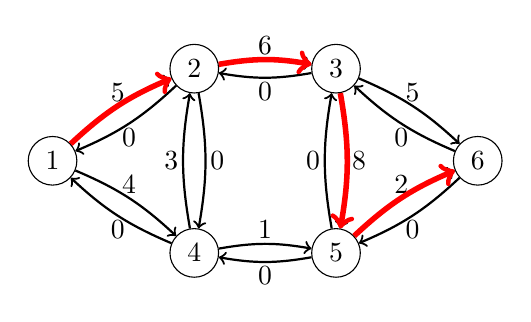
\begin{tikzpicture}[scale=0.9,label distance=-2mm]
\node[draw, circle] (1) at (1,1.3) {$1$};
\node[draw, circle] (2) at (3,2.6) {$2$};
\node[draw, circle] (3) at (5,2.6) {$3$};
\node[draw, circle] (4) at (7,1.3) {$6$};
\node[draw, circle] (5) at (3,0) {$4$};
\node[draw, circle] (6) at (5,0) {$5$};

\path[draw,thick,->] (1) edge [bend left=10] node[font=\small,label=5] {} (2);
\path[draw,thick,->] (2) edge [bend left=10] node[font=\small,label=below:0] {} (1);
\path[draw,thick,->] (2) edge [bend left=10] node[font=\small,label=6] {} (3);
\path[draw,thick,->] (3) edge [bend left=10] node[font=\small,label=below:0] {} (2);
\path[draw,thick,->] (3) edge [bend left=10] node[font=\small,label=5] {} (4);
\path[draw,thick,->] (4) edge [bend left=10] node[font=\small,label=below:0] {} (3);
\path[draw,thick,->] (1) edge [bend left=10] node[font=\small,label=4] {} (5);
\path[draw,thick,->] (5) edge [bend left=10] node[font=\small,label=below:0] {} (1);
\path[draw,thick,->] (5) edge [bend left=10] node[font=\small,label=1] {} (6);
\path[draw,thick,->] (6) edge [bend left=10] node[font=\small,label=below:0] {} (5);
\path[draw,thick,->] (6) edge [bend left=10] node[font=\small,label=2] {} (4);
\path[draw,thick,->] (4) edge [bend left=10] node[font=\small,label=below:0] {} (6);
\path[draw,thick,->] (5) edge [bend left=10] node[font=\small,label=left:3] {} (2);
\path[draw,thick,->] (2) edge [bend left=10] node[font=\small,label=right:0] {} (5);
\path[draw,thick,->] (3) edge [bend left=10] node[font=\small,label=right:8] {} (6);
\path[draw,thick,->] (6) edge [bend left=10] node[font=\small,label=left:0] {} (3);

\path[draw=red,thick,->,line width=2pt] (1) edge [bend left=10] (2);
\path[draw=red,thick,->,line width=2pt] (2) edge [bend left=10] (3);
\path[draw=red,thick,->,line width=2pt] (3) edge [bend left=10] (6);
\path[draw=red,thick,->,line width=2pt] (6) edge [bend left=10] (4);
\end{tikzpicture}
\end{center}

Polun valinnan jälkeen virtaus lisääntyy $x$ yksikköä,
jossa $x$ on pienin kaaren kapasiteetti polulla.
Samalla jokaisen polulla olevan kaaren kapasiteetti
vähenee $x$:llä ja jokaisen käänteisen kaaren kapasiteetti kasvaa $x$:llä.

Yllä valitussa polussa
kaarten kapasiteetit ovat 5, 6, 8 ja 2.
Pienin kapasiteetti on 2,
joten virtaus kasvaa 2:lla
ja verkko muuttuu seuraavasti:

\begin{center}
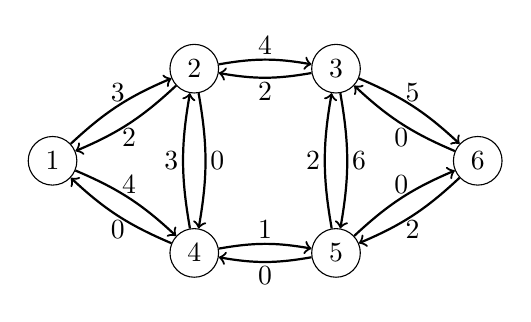
\begin{tikzpicture}[scale=0.9,label distance=-2mm]
\node[draw, circle] (1) at (1,1.3) {$1$};
\node[draw, circle] (2) at (3,2.6) {$2$};
\node[draw, circle] (3) at (5,2.6) {$3$};
\node[draw, circle] (4) at (7,1.3) {$6$};
\node[draw, circle] (5) at (3,0) {$4$};
\node[draw, circle] (6) at (5,0) {$5$};

\path[draw,thick,->] (1) edge [bend left=10] node[font=\small,label=3] {} (2);
\path[draw,thick,->] (2) edge [bend left=10] node[font=\small,label=below:2] {} (1);
\path[draw,thick,->] (2) edge [bend left=10] node[font=\small,label=4] {} (3);
\path[draw,thick,->] (3) edge [bend left=10] node[font=\small,label=below:2] {} (2);
\path[draw,thick,->] (3) edge [bend left=10] node[font=\small,label=5] {} (4);
\path[draw,thick,->] (4) edge [bend left=10] node[font=\small,label=below:0] {} (3);
\path[draw,thick,->] (1) edge [bend left=10] node[font=\small,label=4] {} (5);
\path[draw,thick,->] (5) edge [bend left=10] node[font=\small,label=below:0] {} (1);
\path[draw,thick,->] (5) edge [bend left=10] node[font=\small,label=1] {} (6);
\path[draw,thick,->] (6) edge [bend left=10] node[font=\small,label=below:0] {} (5);
\path[draw,thick,->] (6) edge [bend left=10] node[font=\small,label=0] {} (4);
\path[draw,thick,->] (4) edge [bend left=10] node[font=\small,label=below:2] {} (6);
\path[draw,thick,->] (5) edge [bend left=10] node[font=\small,label=left:3] {} (2);
\path[draw,thick,->] (2) edge [bend left=10] node[font=\small,label=right:0] {} (5);
\path[draw,thick,->] (3) edge [bend left=10] node[font=\small,label=right:6] {} (6);
\path[draw,thick,->] (6) edge [bend left=10] node[font=\small,label=left:2] {} (3);
\end{tikzpicture}
\end{center}

Muutoksessa on ideana, että virtauksen lisääminen
vähentää polkuun kuuluvien kaarten kykyä välittää virtausta.
Toisaalta virtausta on mahdollista peruuttaa myöhemmin
käyttämällä käänteisiä kaaria, jos osoittautuu, että
virtausta on järkevää reitittää verkossa toisella tavalla.

Algoritmi kasvattaa virtausta
niin kauan, kuin verkossa on olemassa polku
alkusolmusta loppusolmuun positiivisia kaaria pitkin.
Tässä tapauksessa
voimme valita seuraavan polun vaikkapa näin:

\begin{center}
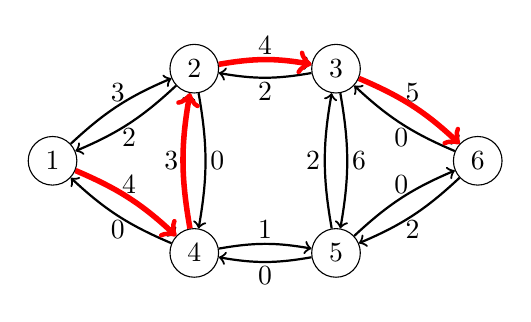
\begin{tikzpicture}[scale=0.9,label distance=-2mm]
\node[draw, circle] (1) at (1,1.3) {$1$};
\node[draw, circle] (2) at (3,2.6) {$2$};
\node[draw, circle] (3) at (5,2.6) {$3$};
\node[draw, circle] (4) at (7,1.3) {$6$};
\node[draw, circle] (5) at (3,0) {$4$};
\node[draw, circle] (6) at (5,0) {$5$};

\path[draw,thick,->] (1) edge [bend left=10] node[font=\small,label=3] {} (2);
\path[draw,thick,->] (2) edge [bend left=10] node[font=\small,label=below:2] {} (1);
\path[draw,thick,->] (2) edge [bend left=10] node[font=\small,label=4] {} (3);
\path[draw,thick,->] (3) edge [bend left=10] node[font=\small,label=below:2] {} (2);
\path[draw,thick,->] (3) edge [bend left=10] node[font=\small,label=5] {} (4);
\path[draw,thick,->] (4) edge [bend left=10] node[font=\small,label=below:0] {} (3);
\path[draw,thick,->] (1) edge [bend left=10] node[font=\small,label=4] {} (5);
\path[draw,thick,->] (5) edge [bend left=10] node[font=\small,label=below:0] {} (1);
\path[draw,thick,->] (5) edge [bend left=10] node[font=\small,label=1] {} (6);
\path[draw,thick,->] (6) edge [bend left=10] node[font=\small,label=below:0] {} (5);
\path[draw,thick,->] (6) edge [bend left=10] node[font=\small,label=0] {} (4);
\path[draw,thick,->] (4) edge [bend left=10] node[font=\small,label=below:2] {} (6);
\path[draw,thick,->] (5) edge [bend left=10] node[font=\small,label=left:3] {} (2);
\path[draw,thick,->] (2) edge [bend left=10] node[font=\small,label=right:0] {} (5);
\path[draw,thick,->] (3) edge [bend left=10] node[font=\small,label=right:6] {} (6);
\path[draw,thick,->] (6) edge [bend left=10] node[font=\small,label=left:2] {} (3);

\path[draw=red,thick,->,line width=2pt] (1) edge [bend left=10] (5);
\path[draw=red,thick,->,line width=2pt] (5) edge [bend left=10] (2);
\path[draw=red,thick,->,line width=2pt] (2) edge [bend left=10] (3);
\path[draw=red,thick,->,line width=2pt] (3) edge [bend left=10] (4);
\end{tikzpicture}
\end{center}

Tämän polun pienin kapasiteetti on 3,
joten polku kasvattaa virtausta 3:lla
ja kokonaisvirtaus polun käsittelyn jälkeen on 5.

\begin{samepage}
Nyt verkko muuttuu seuraavasti:

\begin{center}
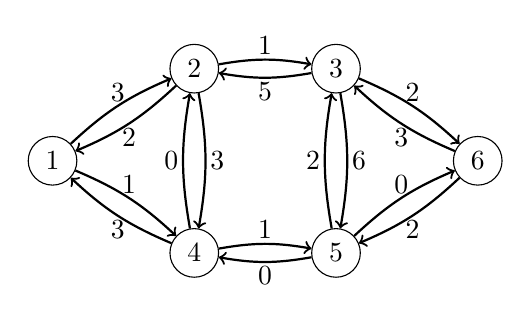
\begin{tikzpicture}[scale=0.9,label distance=-2mm]
\node[draw, circle] (1) at (1,1.3) {$1$};
\node[draw, circle] (2) at (3,2.6) {$2$};
\node[draw, circle] (3) at (5,2.6) {$3$};
\node[draw, circle] (4) at (7,1.3) {$6$};
\node[draw, circle] (5) at (3,0) {$4$};
\node[draw, circle] (6) at (5,0) {$5$};

\path[draw,thick,->] (1) edge [bend left=10] node[font=\small,label=3] {} (2);
\path[draw,thick,->] (2) edge [bend left=10] node[font=\small,label=below:2] {} (1);
\path[draw,thick,->] (2) edge [bend left=10] node[font=\small,label=1] {} (3);
\path[draw,thick,->] (3) edge [bend left=10] node[font=\small,label=below:5] {} (2);
\path[draw,thick,->] (3) edge [bend left=10] node[font=\small,label=2] {} (4);
\path[draw,thick,->] (4) edge [bend left=10] node[font=\small,label=below:3] {} (3);
\path[draw,thick,->] (1) edge [bend left=10] node[font=\small,label=1] {} (5);
\path[draw,thick,->] (5) edge [bend left=10] node[font=\small,label=below:3] {} (1);
\path[draw,thick,->] (5) edge [bend left=10] node[font=\small,label=1] {} (6);
\path[draw,thick,->] (6) edge [bend left=10] node[font=\small,label=below:0] {} (5);
\path[draw,thick,->] (6) edge [bend left=10] node[font=\small,label=0] {} (4);
\path[draw,thick,->] (4) edge [bend left=10] node[font=\small,label=below:2] {} (6);
\path[draw,thick,->] (5) edge [bend left=10] node[font=\small,label=left:0] {} (2);
\path[draw,thick,->] (2) edge [bend left=10] node[font=\small,label=right:3] {} (5);
\path[draw,thick,->] (3) edge [bend left=10] node[font=\small,label=right:6] {} (6);
\path[draw,thick,->] (6) edge [bend left=10] node[font=\small,label=left:2] {} (3);
\end{tikzpicture}
\end{center}
\end{samepage}

Maksimivirtaus tulee valmiiksi
lisäämällä virtausta vielä polkujen $1 \rightarrow 2 \rightarrow 3 \rightarrow 6$ ja
$1 \rightarrow 4 \rightarrow 5 \rightarrow 3 \rightarrow 6$ avulla.
Molemmat polut tuottavat 1 yksikön lisää virtausta,
ja lopullinen verkko on seuraava:

\begin{center}
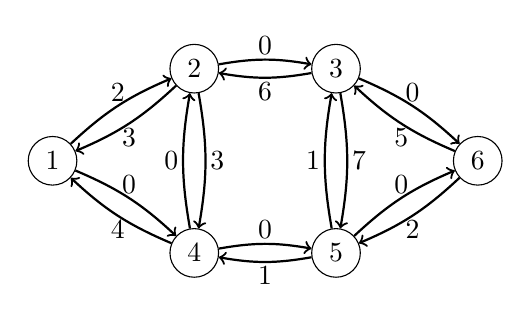
\begin{tikzpicture}[scale=0.9,label distance=-2mm]
\node[draw, circle] (1) at (1,1.3) {$1$};
\node[draw, circle] (2) at (3,2.6) {$2$};
\node[draw, circle] (3) at (5,2.6) {$3$};
\node[draw, circle] (4) at (7,1.3) {$6$};
\node[draw, circle] (5) at (3,0) {$4$};
\node[draw, circle] (6) at (5,0) {$5$};

\path[draw,thick,->] (1) edge [bend left=10] node[font=\small,label=2] {} (2);
\path[draw,thick,->] (2) edge [bend left=10] node[font=\small,label=below:3] {} (1);
\path[draw,thick,->] (2) edge [bend left=10] node[font=\small,label=0] {} (3);
\path[draw,thick,->] (3) edge [bend left=10] node[font=\small,label=below:6] {} (2);
\path[draw,thick,->] (3) edge [bend left=10] node[font=\small,label=0] {} (4);
\path[draw,thick,->] (4) edge [bend left=10] node[font=\small,label=below:5] {} (3);
\path[draw,thick,->] (1) edge [bend left=10] node[font=\small,label=0] {} (5);
\path[draw,thick,->] (5) edge [bend left=10] node[font=\small,label=below:4] {} (1);
\path[draw,thick,->] (5) edge [bend left=10] node[font=\small,label=0] {} (6);
\path[draw,thick,->] (6) edge [bend left=10] node[font=\small,label=below:1] {} (5);
\path[draw,thick,->] (6) edge [bend left=10] node[font=\small,label=0] {} (4);
\path[draw,thick,->] (4) edge [bend left=10] node[font=\small,label=below:2] {} (6);
\path[draw,thick,->] (5) edge [bend left=10] node[font=\small,label=left:0] {} (2);
\path[draw,thick,->] (2) edge [bend left=10] node[font=\small,label=right:3] {} (5);
\path[draw,thick,->] (3) edge [bend left=10] node[font=\small,label=right:7] {} (6);
\path[draw,thick,->] (6) edge [bend left=10] node[font=\small,label=left:1] {} (3);
\end{tikzpicture}
\end{center}

Nyt virtausta ei pysty enää kasvattamaan,
koska verkossa ei ole mitään polkua
alkusolmusta loppusolmuun,
jossa jokaisen kaaren paino olisi positiivinen.
Niinpä algoritmi pysähtyy ja verkon maksimivirtaus on 7.

\subsubsection{Polun valinta}

Ford-Fulkersonin algoritmi ei ota kantaa siihen,
millä tavoin virtausta kasvattava polku valitaan verkossa.
Valintatavasta riippumatta algoritmi pysähtyy
ja tuottaa maksimivirtauksen ennemmin tai myöhemmin,
mutta polun valinnalla on vaikutusta algoritmin tehokkuuteen.

Yksinkertainen tapa on valita virtausta kasvattava
polku syvyyshaulla.
Tämä toimii usein hyvin, mutta pahin tapaus on,
että jokainen polku
kasvattaa virtausta vain 1:llä ja algoritmi toimii hitaasti.
Seuraavaksi käymme läpi kaksi tapaa polun valintaan,
jotka estävät tämän ilmiön.

\textit{Edmonds-Karpin algoritmi} on
Ford-Fulkersonin algoritmin toteutus,
jossa virtausta kasvattava polku valitaan
aina niin, että siinä on mahdollisimman vähän kaaria.
Tämä onnistuu etsimällä polku syvyyshaun
sijasta leveyshaulla.
Osoittautuu, että tämä varmistaa virtauksen
kasvamisen nopeasti ja
maksimivirtauksen etsiminen vie aikaa $O(m^2 n)$.

\textit{Skaalaava algoritmi}
asettaa minimiarvon, joka on ensin alkusolmusta
lähtevien kaarten kapasiteettien summa $c$.
Joka vaiheessa verkosta etsitään
syvyyshaulla polku, jonka jokaisen kaaren kapasiteetti
on vähintään minimiarvo.
Aina jos kelvollista polkua ei löydy,
minimiarvo jaetaan 2:lla,
kunnes lopuksi minimiarvo on 1.
Algoritmin aikavaativuus on $O(m^2 \log c)$.

Käytännössä skaalaava algoritmi on mukavampi koodattava,
koska siinä riittää etsiä polku syvyyshaulla.
Kummatkin algoritmit ovat yleensä aina riittävän
nopeita ohjelmointikisoissa esiintyviin tehtäviin.

\subsubsection{Minimileikkaus}

Osoittautuu, että kun Ford-Fulkersonin algoritmi on saanut valmiiksi
maksimivirtauksen, se on tuottanut samalla minimileikkauksen.
Olkoon $A$ niiden solmujen joukko,
joihin verkossa pääsee
alkusolmusta positiivisia kaaria pitkin.
Esimerkkiverkossa $A$ sisältää solmut 1, 2 ja 4:

\begin{center}
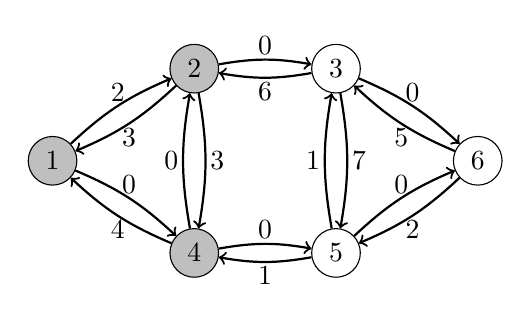
\begin{tikzpicture}[scale=0.9,label distance=-2mm]
\node[draw, circle,fill=lightgray] (1) at (1,1.3) {$1$};
\node[draw, circle,fill=lightgray] (2) at (3,2.6) {$2$};
\node[draw, circle] (3) at (5,2.6) {$3$};
\node[draw, circle] (4) at (7,1.3) {$6$};
\node[draw, circle,fill=lightgray] (5) at (3,0) {$4$};
\node[draw, circle] (6) at (5,0) {$5$};

\path[draw,thick,->] (1) edge [bend left=10] node[font=\small,label=2] {} (2);
\path[draw,thick,->] (2) edge [bend left=10] node[font=\small,label=below:3] {} (1);
\path[draw,thick,->] (2) edge [bend left=10] node[font=\small,label=0] {} (3);
\path[draw,thick,->] (3) edge [bend left=10] node[font=\small,label=below:6] {} (2);
\path[draw,thick,->] (3) edge [bend left=10] node[font=\small,label=0] {} (4);
\path[draw,thick,->] (4) edge [bend left=10] node[font=\small,label=below:5] {} (3);
\path[draw,thick,->] (1) edge [bend left=10] node[font=\small,label=0] {} (5);
\path[draw,thick,->] (5) edge [bend left=10] node[font=\small,label=below:4] {} (1);
\path[draw,thick,->] (5) edge [bend left=10] node[font=\small,label=0] {} (6);
\path[draw,thick,->] (6) edge [bend left=10] node[font=\small,label=below:1] {} (5);
\path[draw,thick,->] (6) edge [bend left=10] node[font=\small,label=0] {} (4);
\path[draw,thick,->] (4) edge [bend left=10] node[font=\small,label=below:2] {} (6);
\path[draw,thick,->] (5) edge [bend left=10] node[font=\small,label=left:0] {} (2);
\path[draw,thick,->] (2) edge [bend left=10] node[font=\small,label=right:3] {} (5);
\path[draw,thick,->] (3) edge [bend left=10] node[font=\small,label=right:7] {} (6);
\path[draw,thick,->] (6) edge [bend left=10] node[font=\small,label=left:1] {} (3);
\end{tikzpicture}
\end{center}

Nyt minimileikkauksen muodostavat ne alkuperäisen verkon kaaret,
jotka kulkevat joukosta $A$ joukon $A$ ulkopuolelle
ja joiden kapasiteetti on täysin käytetty
maksimivirtauksessa.
Tässä verkossa kyseiset kaaret ovat $2 \rightarrow 3$
ja $4 \rightarrow 5$, jotka tuottavat minimileikkauksen $6+1=7$.

Miksi sitten algoritmin tuottama virtaus ja leikkaus ovat
varmasti maksimivirtaus ja minimileikkaus?
Syynä tähän on, että virtauksen suuruus on
\textit{aina} enintään yhtä suuri kuin leikkauksen paino.
Niinpä kun virtaus ja leikkaus ovat yhtä suuret,
ne ovat varmasti maksimivirtaus ja minimileikkaus.

Tarkastellaan mitä tahansa verkon leikkausta,
jossa alkusolmu kuuluu osaan $A$,
loppusolmu kuuluu osaan $B$ ja osien välillä kulkee kaaria:

\begin{center}
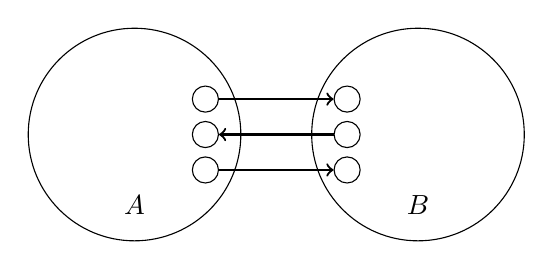
\begin{tikzpicture}[scale=0.9]
\draw (-2,0) circle (1.5);
\draw (2,0) circle (1.5);

\node at (-2,-1) {$A$};
\node at (2,-1) {$B$};

\node[draw, circle] (1) at (-1,0.5) {};
\node[draw, circle] (2) at (-1,0) {};
\node[draw, circle] (3) at (-1,-0.5) {};
\node[draw, circle] (4) at (1,0.5) {};
\node[draw, circle] (5) at (1,0) {};
\node[draw, circle] (6) at (1,-0.5) {};

\path[draw,thick,->] (1) -- (4);
\path[draw,thick,->] (5) -- (2);
\path[draw,thick,->] (3) -- (6);

\end{tikzpicture}
\end{center}

Leikkauksen paino on niiden kaarten painojen summa,
jotka kulkevat osasta $A$ osaan $B$.
Tämä on yläraja sille, kuinka suuri verkossa oleva virtaus voi olla,
koska virtauksen täytyy edetä osasta $A$ osaan $B$.
Niinpä maksimivirtaus on pienempi tai yhtä suuri kuin
mikä tahansa verkon leikkaus.

Toisaalta Ford-Fulkersonin algoritmi tuottaa virtauksen,
joka on tarkalleen yhtä suuri kuin verkossa oleva leikkaus.
Niinpä tämän virtauksen on oltava maksimivirtaus ja
vastaavasti leikkauksen on oltava minimileikkaus.

\section{Rinnakkaiset polut}

Ensimmäisenä virtauslaskennan sovelluksena tarkastelemme
tehtävää, jossa tavoitteena on muodostaa mahdollisimman
monta rinnakkaista polkua verkon alkusolmusta loppusolmuun.
Vaatimuksena on, että jokainen verkon kaari esiintyy
enintään yhdellä polulla.

Esimerkiksi verkossa
\begin{center}
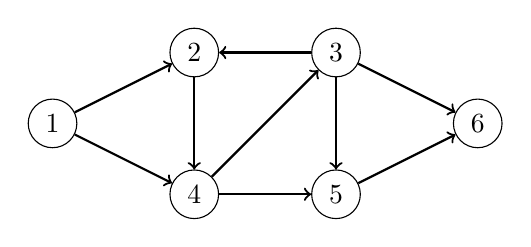
\begin{tikzpicture}[scale=0.9]
\node[draw, circle] (1) at (1,2) {$1$};
\node[draw, circle] (2) at (3,3) {$2$};
\node[draw, circle] (3) at (5,3) {$3$};
\node[draw, circle] (4) at (3,1) {$4$};
\node[draw, circle] (5) at (5,1) {$5$};
\node[draw, circle] (6) at (7,2) {$6$};
\path[draw,thick,->] (1) -- (2);
\path[draw,thick,->] (1) -- (4);
\path[draw,thick,->] (2) -- (4);
\path[draw,thick,->] (3) -- (2);
\path[draw,thick,->] (3) -- (5);
\path[draw,thick,->] (3) -- (6);
\path[draw,thick,->] (4) -- (3);
\path[draw,thick,->] (4) -- (5);
\path[draw,thick,->] (5) -- (6);
\end{tikzpicture}
\end{center}

pystyy muodostamaan kaksi rinnakkaista polkua solmusta 1 solmuun 6.
Tämä toteutuu valitsemalla polut
$1 \rightarrow 2 \rightarrow 4 \rightarrow 3 \rightarrow 6$
ja $1 \rightarrow 4 \rightarrow 5 \rightarrow 6$:

\begin{center}
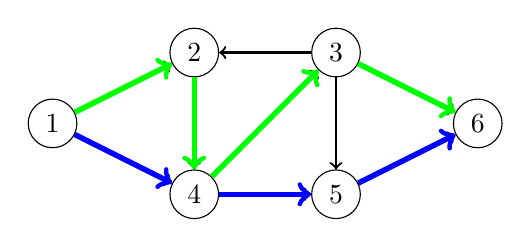
\begin{tikzpicture}[scale=0.9]
\node[draw, circle] (1) at (1,2) {$1$};
\node[draw, circle] (2) at (3,3) {$2$};
\node[draw, circle] (3) at (5,3) {$3$};
\node[draw, circle] (4) at (3,1) {$4$};
\node[draw, circle] (5) at (5,1) {$5$};
\node[draw, circle] (6) at (7,2) {$6$};
\path[draw,thick,->] (1) -- (2);
\path[draw,thick,->] (1) -- (4);
\path[draw,thick,->] (2) -- (4);
\path[draw,thick,->] (3) -- (2);
\path[draw,thick,->] (3) -- (5);
\path[draw,thick,->] (3) -- (6);
\path[draw,thick,->] (4) -- (3);
\path[draw,thick,->] (4) -- (5);
\path[draw,thick,->] (5) -- (6);

\path[draw=green,thick,->,line width=2pt] (1) -- (2);
\path[draw=green,thick,->,line width=2pt] (2) -- (4);
\path[draw=green,thick,->,line width=2pt] (4) -- (3);
\path[draw=green,thick,->,line width=2pt] (3) -- (6);

\path[draw=blue,thick,->,line width=2pt] (1) -- (4);
\path[draw=blue,thick,->,line width=2pt] (4) -- (5);
\path[draw=blue,thick,->,line width=2pt] (5) -- (6);
\end{tikzpicture}
\end{center}

Osoittautuu, että suurin rinnakkaisten polkujen määrä
on yhtä suuri kuin maksimivirtaus verkossa,
jossa jokaisen kaaren kapasiteetti on 1.
Kun maksimivirtaus on muodostettu,
rinnakkaiset polut voi löytää
ahneesti etsimällä alkusolmusta loppusolmuun
kulkevia polkuja.

Tarkastellaan sitten tehtävän muunnelmaa,
jossa jokainen solmu (alku- ja loppusolmuja lukuun ottamatta)
saa esiintyä enintään yhdellä polulla.
Tämän rajoituksen seurauksena äskeisessä verkossa
voi muodostaa vain yhden polun,
koska solmu 4 ei voi esiintyä monella polulla:

\begin{center}
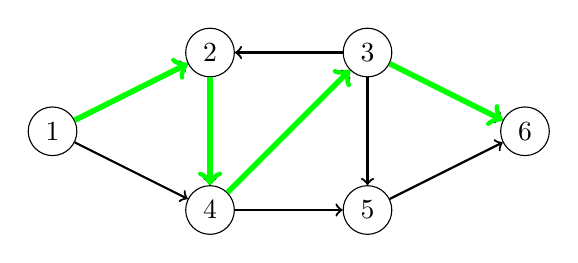
\begin{tikzpicture}
\node[draw, circle] (1) at (1,2) {$1$};
\node[draw, circle] (2) at (3,3) {$2$};
\node[draw, circle] (3) at (5,3) {$3$};
\node[draw, circle] (4) at (3,1) {$4$};
\node[draw, circle] (5) at (5,1) {$5$};
\node[draw, circle] (6) at (7,2) {$6$};
\path[draw,thick,->] (1) -- (2);
\path[draw,thick,->] (1) -- (4);
\path[draw,thick,->] (2) -- (4);
\path[draw,thick,->] (3) -- (2);
\path[draw,thick,->] (3) -- (5);
\path[draw,thick,->] (3) -- (6);
\path[draw,thick,->] (4) -- (3);
\path[draw,thick,->] (4) -- (5);
\path[draw,thick,->] (5) -- (6);

\path[draw=green,thick,->,line width=2pt] (1) -- (2);
\path[draw=green,thick,->,line width=2pt] (2) -- (4);
\path[draw=green,thick,->,line width=2pt] (4) -- (3);
\path[draw=green,thick,->,line width=2pt] (3) -- (6);
\end{tikzpicture}
\end{center}

Tavallinen keino rajoittaa solmun kautta kulkevaa
virtausta on jakaa solmu tulosolmuksi ja lähtösolmuksi.
Kaikki solmuun tulevat kaaret saapuvat tulosolmuun
ja kaikki solmusta lähtevät kaaret poistuvat lähtösolmusta.
Lisäksi tulosolmusta lähtösolmuun on kaari,
jossa on haluttu kapasiteetti.

Tässä tapauksessa verkosta tulee seuraava:
\begin{center}
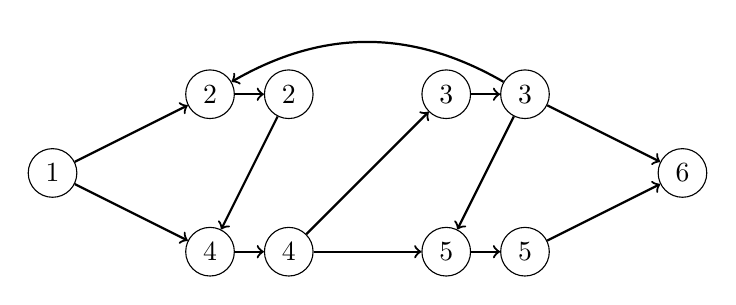
\begin{tikzpicture}
\node[draw, circle] (1) at (1,2) {$1$};

\node[draw, circle] (2a) at (3,3) {$2$};
\node[draw, circle] (3a) at (6,3) {$3$};
\node[draw, circle] (4a) at (3,1) {$4$};
\node[draw, circle] (5a) at (6,1) {$5$};

\node[draw, circle] (2b) at (4,3) {$2$};
\node[draw, circle] (3b) at (7,3) {$3$};
\node[draw, circle] (4b) at (4,1) {$4$};
\node[draw, circle] (5b) at (7,1) {$5$};

\node[draw, circle] (6) at (9,2) {$6$};

\path[draw,thick,->] (2a) -- (2b);
\path[draw,thick,->] (3a) -- (3b);
\path[draw,thick,->] (4a) -- (4b);
\path[draw,thick,->] (5a) -- (5b);

\path[draw,thick,->] (1) -- (2a);
\path[draw,thick,->] (1) -- (4a);
\path[draw,thick,->] (2b) -- (4a);
\path[draw,thick,->] (3b) edge [bend right=30] (2a);
\path[draw,thick,->] (3b) -- (5a);
\path[draw,thick,->] (3b) -- (6);
\path[draw,thick,->] (4b) -- (3a);
\path[draw,thick,->] (4b) -- (5a);
\path[draw,thick,->] (5b) -- (6);
\end{tikzpicture}
\end{center}

Tämän verkon maksimivirtaus on:
\begin{center}
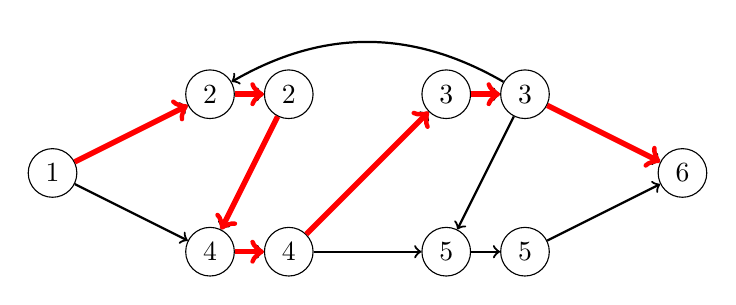
\begin{tikzpicture}
\node[draw, circle] (1) at (1,2) {$1$};

\node[draw, circle] (2a) at (3,3) {$2$};
\node[draw, circle] (3a) at (6,3) {$3$};
\node[draw, circle] (4a) at (3,1) {$4$};
\node[draw, circle] (5a) at (6,1) {$5$};

\node[draw, circle] (2b) at (4,3) {$2$};
\node[draw, circle] (3b) at (7,3) {$3$};
\node[draw, circle] (4b) at (4,1) {$4$};
\node[draw, circle] (5b) at (7,1) {$5$};

\node[draw, circle] (6) at (9,2) {$6$};

\path[draw,thick,->] (2a) -- (2b);
\path[draw,thick,->] (3a) -- (3b);
\path[draw,thick,->] (4a) -- (4b);
\path[draw,thick,->] (5a) -- (5b);

\path[draw,thick,->] (1) -- (2a);
\path[draw,thick,->] (1) -- (4a);
\path[draw,thick,->] (2b) -- (4a);
\path[draw,thick,->] (3b) edge [bend right=30] (2a);
\path[draw,thick,->] (3b) -- (5a);
\path[draw,thick,->] (3b) -- (6);
\path[draw,thick,->] (4b) -- (3a);
\path[draw,thick,->] (4b) -- (5a);
\path[draw,thick,->] (5b) -- (6);

\path[draw=red,thick,->,line width=2pt] (1) -- (2a);
\path[draw=red,thick,->,line width=2pt] (2a) -- (2b);
\path[draw=red,thick,->,line width=2pt] (2b) -- (4a);
\path[draw=red,thick,->,line width=2pt] (4a) -- (4b);
\path[draw=red,thick,->,line width=2pt] (4b) -- (3a);
\path[draw=red,thick,->,line width=2pt] (3a) -- (3b);
\path[draw=red,thick,->,line width=2pt] (3b) -- (6);
\end{tikzpicture}
\end{center}

Tämä tarkoittaa, että verkossa on mahdollista muodostaa
vain yksi polku alkusolmusta lähtösolmuun,
kun sama solmu ei saa esiintyä monessa polussa.

\section{Maksimiparitus}

Verkon paritus (\textit{matching}) on kokoelma kaaria,
jotka on valittu niin, että jokainen verkon solmu
esiintyy enintään yhden paritukseen kuuluvan kaaren päätesolmuna.
Maksimiparitus (\textit{maximum matching})
on puolestaan paritus, jossa parien määrä on mahdollisimman suuri.

Maksimiparituksen etsimiseen yleisessä
verkossa on olemassa polynominen algoritmi,
mutta se on hyvin monimutkainen.
Tässä luvussa keskitymmekin tilanteeseen,
jossa verkko on kaksijakoinen.
Tällöin maksimiparituksen pystyy etsimään
helposti virtauslaskennan avulla.

\subsection{Maksimiparituksen etsiminen}

Kaksijakoinen verkko voidaan esittää aina niin,
että kukin verkon solmu on vasemmalla tai oikealle
puolella ja kaikki verkon kaaret kulkevat puolten välillä.
Tarkastellaan esimerkkinä seuraavaa verkkoa:

\begin{center}
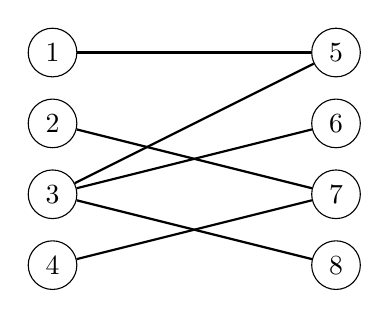
\begin{tikzpicture}[scale=0.60]
\node[draw, circle] (1) at (2,4.5) {1};
\node[draw, circle] (2) at (2,3) {2};
\node[draw, circle] (3) at (2,1.5) {3};
\node[draw, circle] (4) at (2,0) {4};
\node[draw, circle] (5) at (8,4.5) {5};
\node[draw, circle] (6) at (8,3) {6};
\node[draw, circle] (7) at (8,1.5) {7};
\node[draw, circle] (8) at (8,0) {8};

\path[draw,thick,-] (1) -- (5);
\path[draw,thick,-] (2) -- (7);
\path[draw,thick,-] (3) -- (5);
\path[draw,thick,-] (3) -- (6);
\path[draw,thick,-] (3) -- (8);
\path[draw,thick,-] (4) -- (7);
\end{tikzpicture}
\end{center}

Tässä verkossa maksimiparituksen koko on 3:
\begin{center}
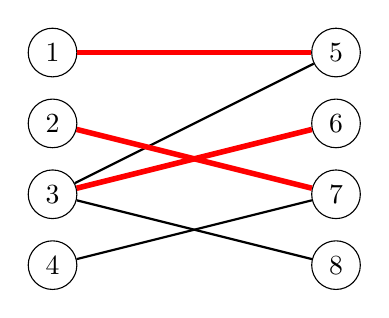
\begin{tikzpicture}[scale=0.60]
\node[draw, circle] (1) at (2,4.5) {1};
\node[draw, circle] (2) at (2,3) {2};
\node[draw, circle] (3) at (2,1.5) {3};
\node[draw, circle] (4) at (2,0) {4};
\node[draw, circle] (5) at (8,4.5) {5};
\node[draw, circle] (6) at (8,3) {6};
\node[draw, circle] (7) at (8,1.5) {7};
\node[draw, circle] (8) at (8,0) {8};

\path[draw,thick,-] (1) -- (5);
\path[draw,thick,-] (2) -- (7);
\path[draw,thick,-] (3) -- (5);
\path[draw,thick,-] (3) -- (6);
\path[draw,thick,-] (3) -- (8);
\path[draw,thick,-] (4) -- (7);

\path[draw=red,thick,-,line width=2pt] (1) -- (5);
\path[draw=red,thick,-,line width=2pt] (2) -- (7);
\path[draw=red,thick,-,line width=2pt] (3) -- (6);
\end{tikzpicture}
\end{center}

Kaksijakoisen verkon maksimiparitus
vastaa aina maksimivirtausta verkossa,
johon on lisätty alkusolmu ja loppusolmu.
Alkusolmusta on kaari jokaiseen vasemman
puolen solmuun, ja vastaavasti loppusolmuun
on kaari jokaisesta oikean puolen solmusta.
Jokaisen kaaren kapasiteettina on 1.

Esimerkissä tuloksena on seuraava verkko:

\begin{center}
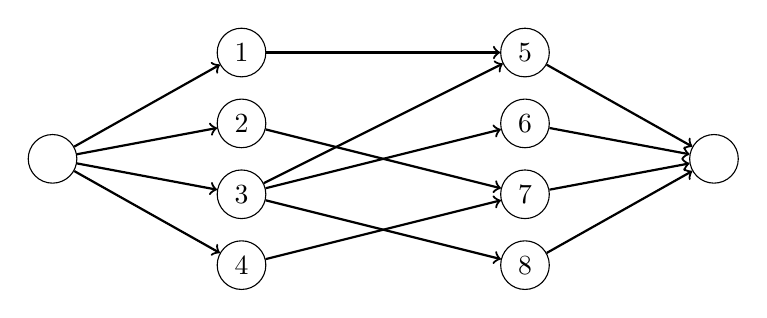
\begin{tikzpicture}[scale=0.60]
\node[draw, circle] (1) at (2,4.5) {1};
\node[draw, circle] (2) at (2,3) {2};
\node[draw, circle] (3) at (2,1.5) {3};
\node[draw, circle] (4) at (2,0) {4};
\node[draw, circle] (5) at (8,4.5) {5};
\node[draw, circle] (6) at (8,3) {6};
\node[draw, circle] (7) at (8,1.5) {7};
\node[draw, circle] (8) at (8,0) {8};

\node[draw, circle] (a) at (-2,2.25) {\phantom{0}};
\node[draw, circle] (b) at (12,2.25) {\phantom{0}};

\path[draw,thick,->] (1) -- (5);
\path[draw,thick,->] (2) -- (7);
\path[draw,thick,->] (3) -- (5);
\path[draw,thick,->] (3) -- (6);
\path[draw,thick,->] (3) -- (8);
\path[draw,thick,->] (4) -- (7);

\path[draw,thick,->] (a) -- (1);
\path[draw,thick,->] (a) -- (2);
\path[draw,thick,->] (a) -- (3);
\path[draw,thick,->] (a) -- (4);
\path[draw,thick,->] (5) -- (b);
\path[draw,thick,->] (6) -- (b);
\path[draw,thick,->] (7) -- (b);
\path[draw,thick,->] (8) -- (b);
\end{tikzpicture}
\end{center}

Tämän verkon maksimivirtaus on yhtä suuri kuin
alkuperäisen verkon maksimiparitus,
koska virtaus muodostuu joukosta polkuja
alkusolmusta loppusolmuun ja jokainen
polku ottaa mukaan uuden kaaren paritukseen.
Tässä tapauksessa maksimivirtaus on 3,
joten maksimiparitus on myös 3.

\subsection{Hallin lause}

Hallin lause antaa ehdon, milloin kaksijakoiseen
verkkoon voidaan muodostaa paritus,
joka sisältää kaikki toisen puolen solmut.
Jos kummallakin puolella on yhtä monta solmua,
Hallin lause kertoo, voidaanko muodostaa
täydellinen paritus (\textit{perfect matching}),
jossa kaikki solmut paritetaan keskenään.

Oletetaan, että haluamme muodostaa parituksen,
johon kuuluvat kaikki vasemman puolen solmut.
Olkoon $X$ jokin joukko vasemman puolen solmuja
ja joukko $f(X)$ ne oikean puolen solmut,
jotka ovat yhteydessä joukon $X$ solmuihin.
Hallin lauseen mukaan paritus on mahdollinen
tarkalleen silloin,
kun mille tahansa joukolle $X$ pätee $|X| \le |f(X)|$.

Tarkastellaan Hallin lauseen merkitystä esimerkkiverkossa.
Valitaan ensin $X=\{1,3\}$, jolloin $f(X)=\{5,6,8\}$:

\begin{center}
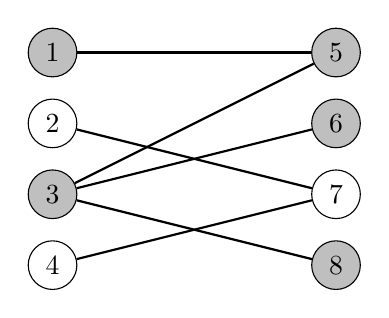
\begin{tikzpicture}[scale=0.60]
\node[draw, circle, fill=lightgray] (1) at (2,4.5) {1};
\node[draw, circle] (2) at (2,3) {2};
\node[draw, circle, fill=lightgray] (3) at (2,1.5) {3};
\node[draw, circle] (4) at (2,0) {4};
\node[draw, circle, fill=lightgray] (5) at (8,4.5) {5};
\node[draw, circle, fill=lightgray] (6) at (8,3) {6};
\node[draw, circle] (7) at (8,1.5) {7};
\node[draw, circle, fill=lightgray] (8) at (8,0) {8};

\path[draw,thick,-] (1) -- (5);
\path[draw,thick,-] (2) -- (7);
\path[draw,thick,-] (3) -- (5);
\path[draw,thick,-] (3) -- (6);
\path[draw,thick,-] (3) -- (8);
\path[draw,thick,-] (4) -- (7);
\end{tikzpicture}
\end{center}

Tämä täyttää Hallin lauseen ehdon, koska $|X|=2$ ja $|f(X)|=3$.
Valitaan sitten $X=\{2,4\}$, jolloin $f(X)=\{7\}$:

\begin{center}
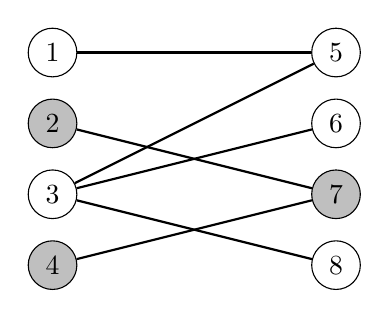
\begin{tikzpicture}[scale=0.60]
\node[draw, circle] (1) at (2,4.5) {1};
\node[draw, circle, fill=lightgray] (2) at (2,3) {2};
\node[draw, circle] (3) at (2,1.5) {3};
\node[draw, circle, fill=lightgray] (4) at (2,0) {4};
\node[draw, circle] (5) at (8,4.5) {5};
\node[draw, circle] (6) at (8,3) {6};
\node[draw, circle, fill=lightgray] (7) at (8,1.5) {7};
\node[draw, circle] (8) at (8,0) {8};

\path[draw,thick,-] (1) -- (5);
\path[draw,thick,-] (2) -- (7);
\path[draw,thick,-] (3) -- (5);
\path[draw,thick,-] (3) -- (6);
\path[draw,thick,-] (3) -- (8);
\path[draw,thick,-] (4) -- (7);
\end{tikzpicture}
\end{center}

Tässä tapauksessa $|X|=2$ ja $|f(X)|=1$, joten Hallin lauseen ehto
ei pidä paikkaansa.
Tämä tarkoittaa, että ei ole mahdollista muodostaa paritusta,
jossa ovat mukana kaikki vasemman puolen solmut
(eli täydellistä paritusta).
Tämä on odotettu tulos, koska verkon maksimiparitus on 3 eikä 4.

Jos Hallin lauseen ehto ei päde, osajoukko $X$
kertoo syyn sille, miksi paritusta ei voi muodostaa.
Koska $X$ sisältää enemmän solmuja kuin $f(X)$,
kaikille $X$:n solmuille ei riitä paria oikealta.
Esimerkiksi yllä molemmat solmut 2 ja 4 tulisi
yhdistää solmuun 7, mutta tämä ei ole mahdollista.

\subsection{Kőnigin lause}

Solmupeite (\textit{vertex cover}) on sellainen joukko
verkon solmuja, että jokaisesta verkon kaaresta ainakin
toinen kaaren päätesolmuista kuuluu joukkoon.
Riippumaton joukko (\textit{independent set})
on puolestaan joukko verkon solmuja,
jossa minkään solmuparin välillä ei ole kaarta.

Jokaista verkon solmupeitettä vastaa riippumaton
joukko, joka muodostuu niistä solmuista,
jotka eivät kuulu solmupeitteeseen.
Niinpä jos verkossa on solmupeite,
jossa on $x$ solmua, niin siinä on myös
riippumaton joukko, jossa on $n-x$ solmua.
Vastaava riippuvuus pätee myös toiseen suuntaan.

Yleisessä verkossa pienimmän solmupeitteen ja
suurimman riippumattoman joukon etsiminen ovat
NP-vaikeita ongelmia.
Kuitenkin kaksijakoisessa verkossa ongelmat ratkeavat tehokkaasti,
koska Kőnigin lauseen nojalla pienin solmupeite on yhtä suurin
kuin maksimiparitus.

Esimerkiksi seuraavan verkon maksimiparituksen koko on 3:

\begin{center}
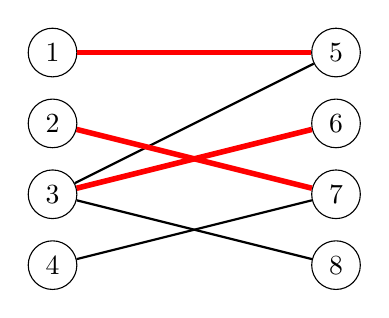
\begin{tikzpicture}[scale=0.60]
\node[draw, circle] (1) at (2,4.5) {1};
\node[draw, circle] (2) at (2,3) {2};
\node[draw, circle] (3) at (2,1.5) {3};
\node[draw, circle] (4) at (2,0) {4};
\node[draw, circle] (5) at (8,4.5) {5};
\node[draw, circle] (6) at (8,3) {6};
\node[draw, circle] (7) at (8,1.5) {7};
\node[draw, circle] (8) at (8,0) {8};

\path[draw,thick,-] (1) -- (5);
\path[draw,thick,-] (2) -- (7);
\path[draw,thick,-] (3) -- (5);
\path[draw,thick,-] (3) -- (6);
\path[draw,thick,-] (3) -- (8);
\path[draw,thick,-] (4) -- (7);

\path[draw=red,thick,-,line width=2pt] (1) -- (5);
\path[draw=red,thick,-,line width=2pt] (2) -- (7);
\path[draw=red,thick,-,line width=2pt] (3) -- (6);
\end{tikzpicture}
\end{center}

Niinpä myös pienimmän solmupeitteen koko on 3.
Solmupeite voidaan muodostaa valitsemalla siihen
solmut $\{1,3,7\}$:

\begin{center}
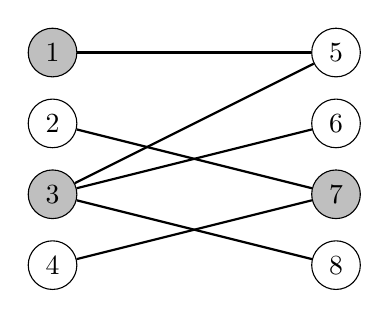
\begin{tikzpicture}[scale=0.60]
\node[draw, circle, fill=lightgray] (1) at (2,4.5) {1};
\node[draw, circle] (2) at (2,3) {2};
\node[draw, circle, fill=lightgray] (3) at (2,1.5) {3};
\node[draw, circle] (4) at (2,0) {4};
\node[draw, circle] (5) at (8,4.5) {5};
\node[draw, circle] (6) at (8,3) {6};
\node[draw, circle, fill=lightgray] (7) at (8,1.5) {7};
\node[draw, circle] (8) at (8,0) {8};

\path[draw,thick,-] (1) -- (5);
\path[draw,thick,-] (2) -- (7);
\path[draw,thick,-] (3) -- (5);
\path[draw,thick,-] (3) -- (6);
\path[draw,thick,-] (3) -- (8);
\path[draw,thick,-] (4) -- (7);
\end{tikzpicture}
\end{center}

Pienin solmupeite muodostuu aina niin,
että jokaisesta maksimiparituksen kaaresta
toinen kaaren päätesolmuista kuuluu peitteeseen.

Pienimmästä solmupeitteestä saadaan suurin
riippumaton joukko valitsemalla
kaikki solmut, jotka eivät kuulu peitteeseen.
Esimerkiksi yllä olevassa verkossa
suurin riippumaton joukko on seuraava:

\begin{center}
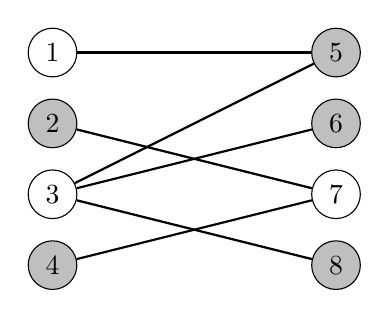
\begin{tikzpicture}[scale=0.60]
\node[draw, circle] (1) at (2,4.5) {1};
\node[draw, circle, fill=lightgray] (2) at (2,3) {2};
\node[draw, circle] (3) at (2,1.5) {3};
\node[draw, circle, fill=lightgray] (4) at (2,0) {4};
\node[draw, circle, fill=lightgray] (5) at (8,4.5) {5};
\node[draw, circle, fill=lightgray] (6) at (8,3) {6};
\node[draw, circle] (7) at (8,1.5) {7};
\node[draw, circle, fill=lightgray] (8) at (8,0) {8};

\path[draw,thick,-] (1) -- (5);
\path[draw,thick,-] (2) -- (7);
\path[draw,thick,-] (3) -- (5);
\path[draw,thick,-] (3) -- (6);
\path[draw,thick,-] (3) -- (8);
\path[draw,thick,-] (4) -- (7);
\end{tikzpicture}
\end{center}

\section{Polkupeitteet}

Polkupeite (\textit{path cover}) on joukko verkon polkuja,
jotka on valittu niin, että jokainen verkon solmu kuuluu
ainakin yhteen polkuun. Seuraavaksi näemme, miten virtauslaskennan
avulla voi etsiä pienimmän polkupeitteen suunnatussa,
syklittömässä verkossa.

Polkupeitteestä on kaksi muunnelmaa:
Solmuerillinen peite on polkupeite,
jossa jokainen verkon solmu esiintyy tasan yhdessä polussa.
Yleinen peite taas on polkupeite, jossa sama solmu voi
esiintyä useammassa polussa.
Kummassakin tapauksessa pienin polkupeite löytyy
samanlaisella idealla.

\subsection{Solmuerillinen peite}

Tarkastellaan esimerkkinä seuraavaa verkkoa:

\begin{center}
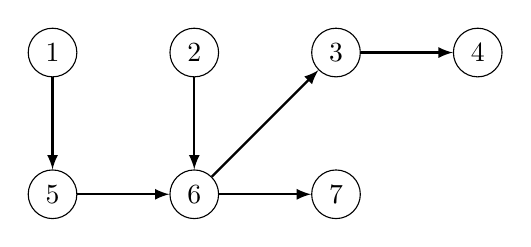
\begin{tikzpicture}[scale=0.9]
\node[draw, circle] (1) at (0,0) {1};
\node[draw, circle] (2) at (2,0) {2};
\node[draw, circle] (3) at (4,0) {3};
\node[draw, circle] (4) at (6,0) {4};
\node[draw, circle] (5) at (0,-2) {5};
\node[draw, circle] (6) at (2,-2) {6};
\node[draw, circle] (7) at (4,-2) {7};

\path[draw,thick,->,>=latex] (1) -- (5);
\path[draw,thick,->,>=latex] (2) -- (6);
\path[draw,thick,->,>=latex] (3) -- (4);
\path[draw,thick,->,>=latex] (5) -- (6);
\path[draw,thick,->,>=latex] (6) -- (3);
\path[draw,thick,->,>=latex] (6) -- (7);
\end{tikzpicture}
\end{center}

Tässä tapauksessa pienin solmuerillinen polkupeite
muodostuu kolmesta polusta.
Voimme valita polut esimerkiksi seuraavasti:

\begin{center}
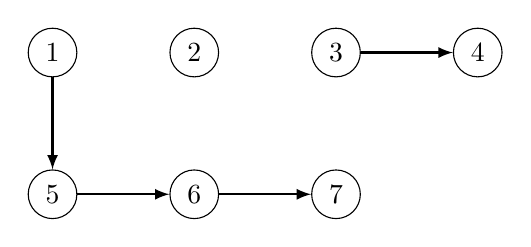
\begin{tikzpicture}[scale=0.9]
\node[draw, circle] (1) at (0,0) {1};
\node[draw, circle] (2) at (2,0) {2};
\node[draw, circle] (3) at (4,0) {3};
\node[draw, circle] (4) at (6,0) {4};
\node[draw, circle] (5) at (0,-2) {5};
\node[draw, circle] (6) at (2,-2) {6};
\node[draw, circle] (7) at (4,-2) {7};

\path[draw,thick,->,>=latex] (1) -- (5);
%\path[draw,thick,->,>=latex] (2) -- (6);
\path[draw,thick,->,>=latex] (3) -- (4);
\path[draw,thick,->,>=latex] (5) -- (6);
%\path[draw,thick,->,>=latex] (6) -- (3);
\path[draw,thick,->,>=latex] (6) -- (7);
\end{tikzpicture}
\end{center}

Huomaa, että yksi poluista sisältää vain solmun 2,
eli on sallittua, että polussa ei ole kaaria.

Polkupeitteen etsiminen voidaan tulkita paritusongelmana
verkossa, jossa jokaista alkuperäisen verkon solmua
vastaa kaksi solmua: vasen ja oikea solmu.
Vasemmasta solmusta oikeaan solmuun on kaari,
jos tällainen kaari esiintyy alkuperäisessä verkossa.
Ideana on, että paritus määrittää, mitkä solmut
ovat yhteydessä toisiinsa poluissa.

Esimerkkiverkossa tilanne on seuraava:

\begin{center}
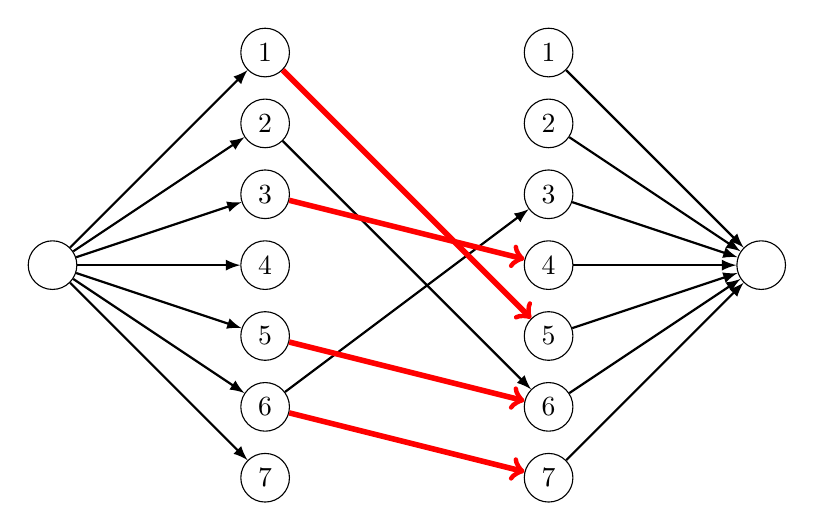
\begin{tikzpicture}[scale=0.9]
\node[draw, circle] (1a) at (0,6) {1};
\node[draw, circle] (2a) at (0,5) {2};
\node[draw, circle] (3a) at (0,4) {3};
\node[draw, circle] (4a) at (0,3) {4};
\node[draw, circle] (5a) at (0,2) {5};
\node[draw, circle] (6a) at (0,1) {6};
\node[draw, circle] (7a) at (0,0) {7};

\node[draw, circle] (1b) at (4,6) {1};
\node[draw, circle] (2b) at (4,5) {2};
\node[draw, circle] (3b) at (4,4) {3};
\node[draw, circle] (4b) at (4,3) {4};
\node[draw, circle] (5b) at (4,2) {5};
\node[draw, circle] (6b) at (4,1) {6};
\node[draw, circle] (7b) at (4,0) {7};

\node[draw, circle] (a) at (-3,3) {\phantom{0}};
\node[draw, circle] (b) at (7,3) {\phantom{0}};

%\path[draw,thick,->,>=latex] (1a) -- (5b);
\path[draw,thick,->,>=latex] (2a) -- (6b);
%\path[draw,thick,->,>=latex] (3a) -- (4b);
%\path[draw,thick,->,>=latex] (5a) -- (6b);
\path[draw,thick,->,>=latex] (6a) -- (3b);
%\path[draw,thick,->,>=latex] (6a) -- (7b);

\path[draw,thick,->,>=latex] (a) -- (1a);
\path[draw,thick,->,>=latex] (a) -- (2a);
\path[draw,thick,->,>=latex] (a) -- (3a);
\path[draw,thick,->,>=latex] (a) -- (4a);
\path[draw,thick,->,>=latex] (a) -- (5a);
\path[draw,thick,->,>=latex] (a) -- (6a);
\path[draw,thick,->,>=latex] (a) -- (7a);

\path[draw,thick,->,>=latex] (1b) -- (b);
\path[draw,thick,->,>=latex] (2b) -- (b);
\path[draw,thick,->,>=latex] (3b) -- (b);
\path[draw,thick,->,>=latex] (4b) -- (b);
\path[draw,thick,->,>=latex] (5b) -- (b);
\path[draw,thick,->,>=latex] (6b) -- (b);
\path[draw,thick,->,>=latex] (7b) -- (b);

\path[draw=red,thick,->,line width=2pt] (1a) -- (5b);
\path[draw=red,thick,->,line width=2pt] (5a) -- (6b);
\path[draw=red,thick,->,line width=2pt] (6a) -- (7b);
\path[draw=red,thick,->,line width=2pt] (3a) -- (4b);

\end{tikzpicture}
\end{center}

Tässä tapauksessa maksimiparitukseen kuuluu neljä kaarta,
jotka vastaavat alkuperäisen verkon kaaria
$1 \rightarrow 5$, $3 \rightarrow 4$,
$5 \rightarrow 6$ ja $6 \rightarrow 7$.
Niinpä pienin solmuerillinen polkupeite syntyy muodostamalla
polut kyseisten kaarten avulla.

Pienimmän polkupeitteen koko on $n-c$, jossa $n$ on verkon
solmujen määrä ja $c$ on maksimiparituksen kaarten määrä.
Esimerkiksi yllä olevassa verkossa pienimmän
polkupeitteen koko on $7-4=3$.

\subsection{Yleinen peite}

Yleisessä polkupeitteessä sama solmu voi kuulua moneen polkuun,
minkä ansiosta tarvittava polkujen määrä saattaa olla pienempi.
Esimerkkiverkossa pienin yleinen polkupeite muodostuu
kahdesta polusta seuraavasti:

\begin{center}
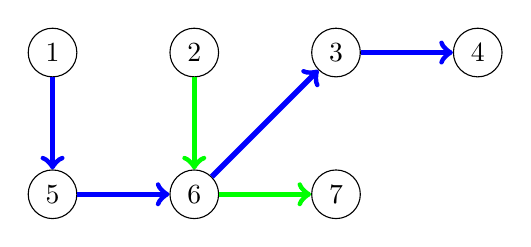
\begin{tikzpicture}[scale=0.9]
\node[draw, circle] (1) at (0,0) {1};
\node[draw, circle] (2) at (2,0) {2};
\node[draw, circle] (3) at (4,0) {3};
\node[draw, circle] (4) at (6,0) {4};
\node[draw, circle] (5) at (0,-2) {5};
\node[draw, circle] (6) at (2,-2) {6};
\node[draw, circle] (7) at (4,-2) {7};

\path[draw=blue,thick,->,line width=2pt] (1) -- (5);
\path[draw=blue,thick,->,line width=2pt] (5) -- (6);
\path[draw=blue,thick,->,line width=2pt] (6) -- (3);
\path[draw=blue,thick,->,line width=2pt] (3) -- (4);
\path[draw=green,thick,->,line width=2pt] (2) -- (6);
\path[draw=green,thick,->,line width=2pt] (6) -- (7);
\end{tikzpicture}
\end{center}

Tässä verkossä yleisessä polkupeitteessä on 2 polkua,
kun taas solmuerillisessä polkupeitteessä on 3 polkua.
Erona on, että yleisessä polkupeitteessä solmua 6
käytetään kahdessa polussa.

Yleisen polkupeitteen voi löytää lähes samalla
tavalla kuin solmuerillisen polkupeitteen.
Riittää täydentää maksimiparituksen verkkoa niin,
että siinä on kaari $a \rightarrow b$ aina silloin,
kun alkuperäisessä verkossa solmusta $a$ pääsee
solmuun $b$ (mahdollisesti usean kaaren kautta).

\subsection{Dilworthin lause}

Dilworthin lauseen mukaan suunnatun, syklittömän
verkon pienin yleinen polkupeite
on yhtä suuri kuin suurin
mahdollinen kokoelma solmuja,
jossa minkään kahden solmun välillä ei ole polkua.

Esimerkiksi äskeisessä verkossa pienin
yleinen polkupeite sisältää kaksi polkua.
Niinpä verkosta voidaan valita enintään kaksi
solmua niin, että minkään solmujen välillä ei ole polkua.
Vaihtoehtoja valintaan on monia: voimme valita esimerkiksi
solmut 3 ja 7:

\begin{center}
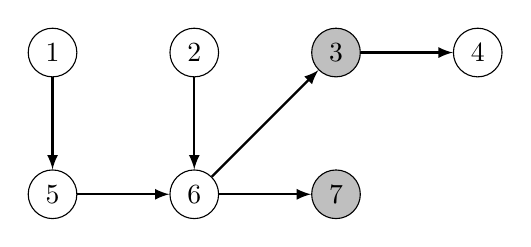
\begin{tikzpicture}[scale=0.9]
\node[draw, circle] (1) at (0,0) {1};
\node[draw, circle] (2) at (2,0) {2};
\node[draw, circle, fill=lightgray] (3) at (4,0) {3};
\node[draw, circle] (4) at (6,0) {4};
\node[draw, circle] (5) at (0,-2) {5};
\node[draw, circle] (6) at (2,-2) {6};
\node[draw, circle, fill=lightgray] (7) at (4,-2) {7};

\path[draw,thick,->,>=latex] (1) -- (5);
\path[draw,thick,->,>=latex] (2) -- (6);
\path[draw,thick,->,>=latex] (3) -- (4);
\path[draw,thick,->,>=latex] (5) -- (6);
\path[draw,thick,->,>=latex] (6) -- (3);
\path[draw,thick,->,>=latex] (6) -- (7);
\end{tikzpicture}
\end{center}

Verkossa ei ole polkua solmusta 3 solmuun 7
eikä polkua solmusta 7 solmuun 3,
joten valinta on kelvollinen.
Toisaalta jos verkosta valitaan mitkä tahansa
kolme solmua, jostain solmusta toiseen on polku.